\documentclass[12pt,a4paper]{scrartcl}
\usepackage[T2A]{fontenc}
\usepackage[utf8]{inputenc}
\usepackage[english,russian]{babel}
\usepackage{indentfirst}
\usepackage{graphicx}
\usepackage{amsmath}
\usepackage[left=2.5cm, right=1.5cm, top=2.5cm, bottom=2.5cm]{geometry}
\usepackage{listings}

\lstloadlanguages{ [LaTeX ] TeX, C++}
\lstset{language=C++,
extendedchars=true,
basicstyle=\small,
frame=tb ,
commentstyle=\itshape ,
stringstyle=\bfseries}


\begin{document}
	\begin{titlepage}
		\begin{center}
		\large
		Государственное образовательное учреждение высшего профессионального образования\\
		“Московский государственный технический университет имени Н.Э.Баумана”
		\vspace{0.25cm}
		
		
		\textsc{Дисциплина: Анализ алгоритмов}\\[5mm]
		\vfill
			
		\textsc{Лабораторная работа № 2}\\[5mm]
		
		{\LARGE Перемножение матриц}
		\bigskip
		
			
		Бутолин Александр Алексеевич\\
		Студент группы ИУ7-52
		\vfill		
		
		\end{center}
		\begin{center}
			2018 г.
		\end{center}
	\end{titlepage}

	

\begin{center}
	\textbf{Введение}
	\label{sec:intro}
\end{center}

В связи с возрастающей потребностью решать задачи, связанные с обработкой матриц, такие как расчет новых координат тела в пространстве, растет необходимость в эффективных алгоритмах по работе с ними. 
Перемножение матриц - одна из стандартных и наиболее используемых операций над матрицами, поэтому существует несколько алгоритмов, позволяющих произвести подобные вычисления. 
В данной работе требуется рассмотреть классический алгоритм и алгоритм Винограда для умножения матриц, а также провести их сравнительный анализ.

Цель работы: изучить алгоритмы умножения матриц (классический и Винограда), а также провести сравнительный анализ. 

Задачи: 

\begin{enumerate}
	\item {Реализовать алгоритмы: классическое умножение матриц, умножение алгоритмом Винограда, умножение улучшенным алгоритмом Винограда; }
	\item {Провести замеры скорости выполнения алгоритмов;} 
	\item {Провести замеры памяти; }
	\item {Описать и обосновать полученные результаты в отчете о выполненной лабораторной работе.}
\end{enumerate}

\newpage
\section{Аналитический раздел}
\label{sec:analitics}

В этом разделе описаны алгоритмы, использованные в данной лабораторной работе.

\subsection{Описание алгоритмов}
\label{sec:analitics:alg}

Умножение матриц — одна из основных операций над матрицами.
Матрица, получаемая в результате операции умножения, называется их произведением. 
Рассмотрим стандартный алгоритм перемножения двух матриц.
Пусть есть две матрицы A и B размера $a\cdot b$ и $c\cdot d$ соответственно. 
Тогда, результатом из умножения будет матрица C размером $a\cdot d$, имеющая вид(\ref{eq:prodresult}):

\begin{equation}\label{eq:prodresult}
\begin{bmatrix}
 c_{11} & c_{12} & \dots & c_{1d} \\
 c_{21} & c_{22} & \dots & c_{2d} \\
 \hdotsfor{4}\\
 c_{a1} & c_{a2} & \dots & c_{ad} \\
\end{bmatrix}
\end{equation}


Каждый элемент матрицы (\ref{eq:prodresult}) представляет собой скалярное произведение соответствующих строки и столбца исходных матриц. 
Часть вычислений можно просчитать заранее. 
Рассмотрим два вектора: 

\begin{equation}\label{eq:vector1}
V = (v_1, v_2, v_3, v_4)
\end{equation}

и

\begin{equation}\label{eq:vector2}
W = (w_1, w_2, w_3, w_4)
\end{equation}


Их скалярное произведение: 

\begin{equation}\label{eq:scalar1}
V * W = v_1 \cdot w_1 + v_2 \cdot w_2 + v_3 \cdot w_3 + v_4 \cdot w_4.
\end{equation}


Это равенство можно переписать в виде: 

\begin{equation}\label{eq:scalar2}
V * W = (v_1 + w_2) \cdot (v_2 + w_1) + (v_3 + w_4) \cdot (v_4 + w_3) - v_1 \cdot v_2 - v_3 \cdot v_4 - w_1 \cdot w_2 - w_3 \cdot w_4
\end{equation}

Несмотря на то, что выражение (\ref{eq:scalar2}) требует больше вычисления, чем (\ref{eq:scalar1}), выражение в правой части последнего равенства (\ref{eq:scalar2}) допускает предварительную обработку. 
Части этого выражения можно вычислить заранее и запомнить для каждой строки первой матрицы и для каждого столбца второй, что позволяет выполнять для каждого элемента лишь первые два умножения и последующие пять сложений, а также дополнительно два сложения.
В этом и заключается алгоритм Винограда.\\ 

В настоящее время умножение матриц активно применяется при решения задач:

\begin{enumerate}
	\item {Касающихся машинного обучения; }
	\item {Преобразования координат тела на плоскости или в пространстве.} 	
\end{enumerate}

\subsection{Вывод}
\label{sec:analitics:conclusion}

Существует несколько возможных алгоритмов перемножения матриц. Это дает возможность произвести их сравнение для определения их преимуществ и недостатков.

\newpage
\section{Конструкторский раздел}
\label{sec:construct}

Сложность стандартного перемножения матриц: O($n^3$)


Для реализации алгоритмов были проведены следующие действия.

\subsection{Схемы алгоритмов}
\label{sec:construct:schemes}

На рисунках представлены схемы реализуемых алгоритмов.

\begin{center}
	\centering
	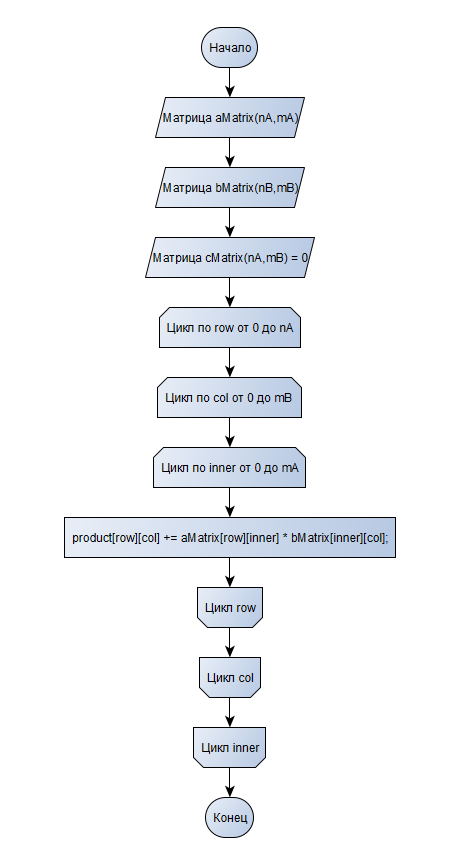
\includegraphics[width=10cm]{multmatrix}\\
	\captionof {figure}{Классический алгоритм перемножения матриц}
	\label{fig:first}
\end{center}


\begin{center}
	\centering
	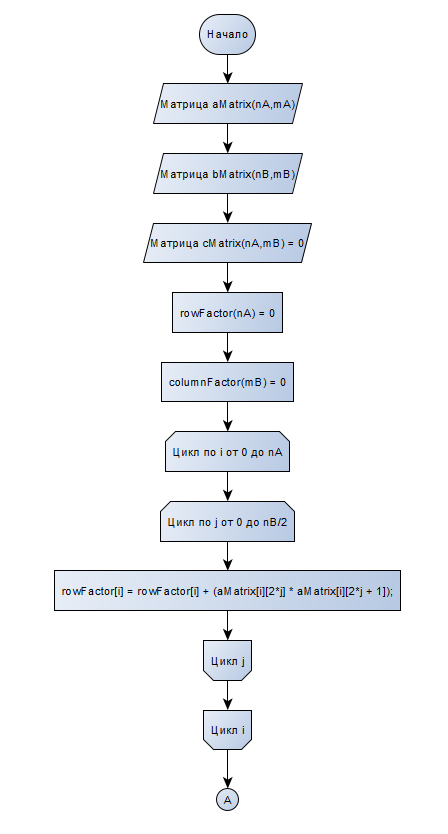
\includegraphics[width=10cm]{multimatrixvinograd1}\\
	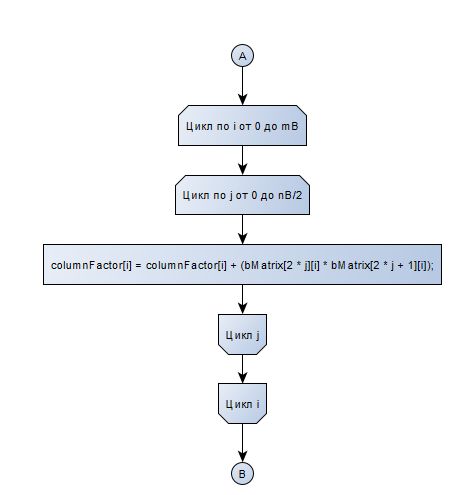
\includegraphics[width=10cm]{multimatrixvinograd2}\\
	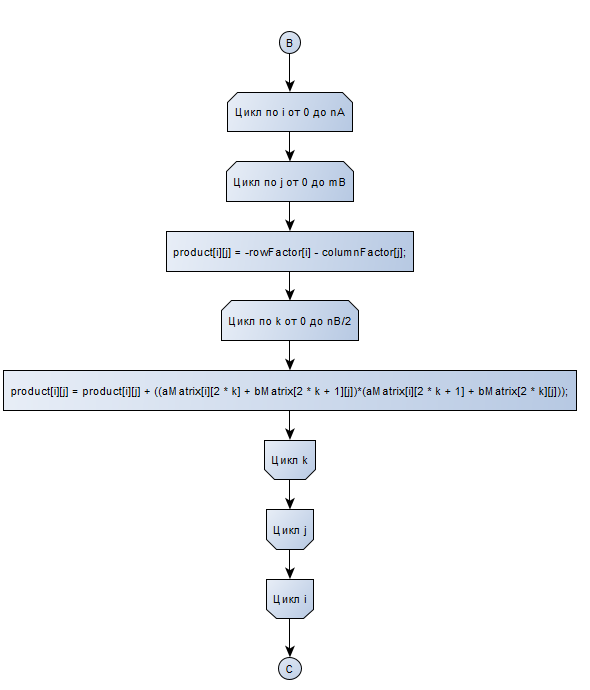
\includegraphics[width=10cm]{multimatrixvinograd3}\\
	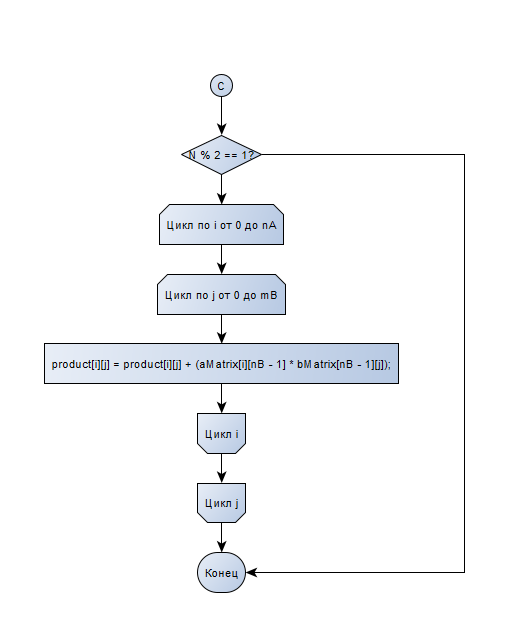
\includegraphics[width=10cm]{multimatrixvinograd4}\\
	\captionof {figure}{Алгоритм Винограда перемножения матриц}
	\label{fig:second}
\end{center}


\newpage
\subsection{Сравнительный анализ стандартного алгоритма перемножения матриц и алгоритма Винограда}
\label{sec:construct:compare}

 Как видно из Рис. \ref{fig:second} алгоритм Винограда можно оптимизировать, так как некоторые операции можно вычислять заранее. 
 Если же сравнивать с классическим алгоритмом, можно сделать предположение, что алгоритм Винограда будет работать медленнее, чем стандартный, из-за наличия дополнительных циклов. 
Так же, алгоритм Винограда использует дополнительные массивы, что должно увеличить объем потребляемой памяти.
Однако можно улучшить алгоритм Винограда путём использования побитового сдвига при обращении к элементам массива, замены оператора a = a + c на a += c и объединения последних двух вложенных циклов в один условный оператор.

\newpage
\section{Технологический раздел}
\label{sec:tech}

В данном разделе будет приведена информация о конкретной реализации приведенных выше алгоритмов, а также исходный код полученных методов.


\subsection{Требования к программному обеспечению}
\label{sec:tech:demands}

К программному обеспечению предъявлены следующие требования:
\begin{enumerate}
\item{Возможность ввода матриц;}
\item{Возможность вывода результатов всех трех алгоритмов;}
\item{Возможность вывода замеров времени, затраченного на работу алгоритмов.}
\end{enumerate}

\subsection{Средства реализации}
\label{sec:tech:relise}

Лабораторная работа была выполнена в VisualStudio2017 на языке C++(c17) \#. 
Замеры процессорного времени были произведены с помощью библиотеки intrin.h.

\subsection{Листинг кода}
\label{sec:tech:listing}

Ниже приведены листинги реализованных методов.

\lstinputlisting[language=C++]{multiply.cpp}
 
\section{Экспериментальная часть}
\label{sec:exp}

При реализации алгоритмов была произведена проверка правильности работы. 
Также был поставлен эксперимент для подтверждения утверждения о том, что алгоритм Винограда работает медленнее классического.

\subsection{Примеры работы}
\label{sec:exp:examples}

Были проведены тесты всех трех алгоритмов для определения правильности их работы.

Тест 1. Умножение.

Матрицы для перемножения:

\begin{minipage}[c][3cm][c]{0,5\textwidth}
	\begin{math}\label{eq:test11}
	A =\begin{bmatrix}
	1 & 2 & 3\\
	-1 & 0 & 10\\
	0 & 0 & 0
	\end{bmatrix}
	\end{math}
\end{minipage}
\begin{minipage}[c][3cm][c]{0,5\textwidth}
	\begin{math}\label{eq:test12}
	B =\begin{bmatrix}
	2 & 4 & 0\\
	5 & 0 & -1\\
	0 & 1 & -1
	\end{bmatrix}
	\end{math}
\end{minipage}

Ожидаемый результат:

\begin{center}
		\begin{math}\label{eq:res1}
		C =\begin{bmatrix}
		12 & 7 & -5\\
		-2 & 6 & -10\\
		0 & 0 & 0
		\end{bmatrix}
		\end{math}
\end{center}

Результаты, где (\ref{eq:res11}) - классический алгоритм, (\ref{eq:res12}) - алгоритм Винограда, и (\ref{eq:res13}) - оптимизированный алгоритм Винограда:

\begin{center}
	\begin{minipage}[c][3cm][c]{0,3\textwidth}
		\begin{equation}\label{eq:res11}
		Classic =\begin{bmatrix}
		12 & 7 & -5\\
		-2 & 6 & -10\\
		0 & 0 & 0
		\end{bmatrix}
		\end{equation}
	\end{minipage}
	\begin{minipage}[c][3cm][c]{0,3\textwidth}
		\begin{equation}\label{eq:res12}
		Winogr =\begin{bmatrix}
		12 & 7 & -5\\
		-2 & 6 & -10\\
		0 & 0 & 0
		\end{bmatrix}
		\end{equation}
	\end{minipage}
	\begin{minipage}[c][3cm][c]{0,3\textwidth}
		\begin{equation}\label{eq:res13}
		WinOpt =\begin{bmatrix}
		12 & 7 & -5\\
		-2 & 6 & -10\\
		0 & 0 & 0
		\end{bmatrix}
		\end{equation}
	\end{minipage}
\end{center}

Тест 2. Умножение на единичную матрицу.

Матрицы для перемножения:

\begin{minipage}[c][3cm][c]{0,5\textwidth}
	\begin{math}\label{eq:test21}
	A =\begin{bmatrix}
	1 & 0 \\
	0 & 1
	\end{bmatrix}
	\end{math}
\end{minipage}
\begin{minipage}[c][3cm][c]{0,5\textwidth}
	\begin{math}\label{eq:test22}
	B =\begin{bmatrix}
	2 & 4 \\
	5 & 0 
	\end{bmatrix}
	\end{math}
\end{minipage}

Ожидаемый результат:

\begin{center}
		\begin{math}\label{eq:res2}
		C =\begin{bmatrix}
		2 & 4 \\
		5 & 0
		\end{bmatrix}
		\end{math}
\end{center}

Результаты, где (\ref{eq:res21}) - классический алгоритм, (\ref{eq:res22}) - алгоритм Винограда, и (\ref{eq:res23}) - оптимизированный алгоритм Винограда:

\begin{center}
	\begin{minipage}[c][3cm][c]{0,3\textwidth}
		\begin{equation}\label{eq:res21}
		Classic =\begin{bmatrix}
		2 & 4 \\ 
		5 & 0
		\end{bmatrix}
		\end{equation}
	\end{minipage}	
	\begin{minipage}[c][3cm][c]{0,3\textwidth}
		\begin{equation}\label{eq:res22}
		Winogr =\begin{bmatrix}
		2 & 4 \\
		5 & 0
		\end{bmatrix}
		\end{equation}
	\end{minipage}	
	\begin{minipage}[c][3cm][c]{0,3\textwidth}
		\begin{equation}\label{eq:res23}
		WinOpt =\begin{bmatrix}
		2 & 4 \\ 
		5 & 0
		\end{bmatrix}
		\end{equation}
	\end{minipage}
\end{center}


Тест 3. Умножение на нулевую матрицу.

Матрицы для перемножения:

\begin{minipage}[c][3cm][c]{0,5\textwidth}
	\begin{math}\label{eq:test31}
	A =\begin{bmatrix}
	-1 & 10 \\
	2 & 1
	\end{bmatrix}
	\end{math}
\end{minipage}
\begin{minipage}[c][3cm][c]{0,5\textwidth}
	\begin{math}\label{eq:test32}
	B =\begin{bmatrix}
	0 & 0 \\
	0 & 0 
	\end{bmatrix}
	\end{math}
\end{minipage}

Ожидаемый результат:

\begin{center}
		\begin{math}\label{eq:res3}
		C =\begin{bmatrix}
		0 & 0 \\
		0 & 0 
		\end{bmatrix}
		\end{math}
\end{center}

Результаты, где (\ref{eq:res31}) - классический алгоритм, (\ref{eq:res32}) - алгоритм Винограда, и (\ref{eq:res33}) - оптимизированный алгоритм Винограда:

\begin{center}
	\begin{minipage}[c][3cm][c]{0,3\textwidth}
		\begin{equation}\label{eq:res31}
		Classic =\begin{bmatrix}
		0 & 0 \\
		0 & 0 
		\end{bmatrix}
		\end{equation}
	\end{minipage}	
	\begin{minipage}[c][3cm][c]{0,3\textwidth}
		\begin{equation}\label{eq:res32}
		Winogr =\begin{bmatrix}
		0 & 0 \\
		0 & 0 
		\end{bmatrix}
		\end{equation}
	\end{minipage}	
	\begin{minipage}[c][3cm][c]{0,3\textwidth}
		\begin{equation}\label{eq:res33}
		WinOpt =\begin{bmatrix}
		0 & 0 \\
		0 & 0 
		\end{bmatrix}
		\end{equation}
	\end{minipage}
\end{center}

Тест 4. Умножение матриц 1x1.

Матрицы для перемножения:

\begin{minipage}[c][3cm][c]{0,5\textwidth}
	\begin{math}\label{eq:test41}
	A =\begin{bmatrix}
	-1
	\end{bmatrix}
	\end{math}
\end{minipage}
\begin{minipage}[c][3cm][c]{0,5\textwidth}
	\begin{math}\label{eq:test42}
	B =\begin{bmatrix}
	2 
	\end{bmatrix}
	\end{math}
\end{minipage}

Ожидаемый результат:

\begin{center}
		\begin{math}\label{eq:res4}
		C =\begin{bmatrix}
		-2 
		\end{bmatrix}
		\end{math}
\end{center}

Результаты, где (\ref{eq:res41}) - классический алгоритм, (\ref{eq:res42}) - алгоритм Винограда, и (\ref{eq:res43}) - оптимизированный алгоритм Винограда:

\begin{center}
	\begin{minipage}[c][3cm][c]{0,3\textwidth}
		\begin{equation}\label{eq:res41}
		Classic =\begin{bmatrix}
		-2 
		\end{bmatrix}
		\end{equation}
	\end{minipage}	
	\begin{minipage}[c][3cm][c]{0,3\textwidth}
		\begin{equation}\label{eq:res42}
		Winogr =\begin{bmatrix}
		-2 
		\end{bmatrix}
		\end{equation}
	\end{minipage}	
	\begin{minipage}[c][3cm][c]{0,3\textwidth}
		\begin{equation}\label{eq:res43}
		WinOpt =\begin{bmatrix}
		-2
		\end{bmatrix}
		\end{equation}
	\end{minipage}
\end{center}

\newpage
\subsection{Постановка эксперимента}
\label{sec:exp:setting}
Замеры времени выполнялся на квадратных матрицах размера от 100x100 до 1000x1000 с шагом 100 для четной совпадающей размерности матриц, и от 101x101 до 1001x1001 для нечетной. 
Числа в матрицах генерировались случайным образом. 

\newpage
\subsection{Сравнительный анализ на основе экспериментальных данных}
\label{sec:exp:compare}

В ходе эксперимента были получены следующие данные, представленные в таблицах 1 и 2.
\\

\begin {flushright}
	Tаблица 1
\end {flushright}
\null \hfill Время выполнения алгоритмов (тики) для четной совпадающей размерности матриц
\begin{table}[ht]
	\label{time2}
	\centering
	\begin{tabular}{|r|r|r|r|}          
		\cline{1-4} & {Классический} & {Виноград} & {Оптимизированный Виноград} \\
		\hline $100$ &	2265522496 & 2191283674 & 1839756105\\
		\hline $200$ &	18050721239 & 17157721168 & 14385504825\\
		\hline $300$ & 61085438711 & 57864873949 & 48365939262\\
		\hline $400$ &	144404496803 & 136729162879 & 114924244078\\
		\hline $500$ &	280343572072 & 265272323038 & 222117101203\\
		\hline $600$ &	454419916713 & 468634129865 & 401878517779\\
		\hline $700$ &	727826428503 & 749552179893 & 616871235096\\
		\hline $800$ &	1077996503537 & 1108881350759 & 920487039006\\
		\hline $900$ &	1537402124157 & 1579516929324 & 1311851684624\\
		\hline $1000$ & 2116661239335 & 2174911323641 & 1808386641669\\
		\hline
	\end{tabular}
\end{table}
\\
\begin {flushright}
	Tаблица 2
\end {flushright}
\null \hfill Время выполнения алгоритмов (тики) для нечетной совпадающей размерности матриц
\begin{table}[ht]
	\label{time1}
	\centering
	\begin{tabular}{|r|r|r|r|}         
		\cline{1-4} & {Классический} & {Виноград} & {Оптимизированный Виноград} \\
		\hline $101$ &	2386501394 & 2227751207 & 1858600569\\
		\hline $201$ &	18301399540 & 17475126873 & 14866810382\\
		\hline $301$ & 61521489095 & 58313321263 & 48771905492\\
		\hline $401$ &	145427694448 & 139823847963 & 116094472809\\
		\hline $501$ &	265299403461 & 272700662438 & 226141044118\\
		\hline $601$ &	457003063880 & 470818479006 & 390446446278\\
		\hline $701$ &	724576583594 & 745894605863 & 619565551412\\
		\hline $801$ &	1082851897339 & 1113222144388 & 925093898256\\
		\hline $901$ & 1540592533368 & 1586115321978 & 1315880047558\\
		\hline
	\end{tabular}
\end{table}


По полученным данным были построены графики, представленные на рисунках \ref{fig:time1} и \ref{fig:time2}.

\begin{center}
	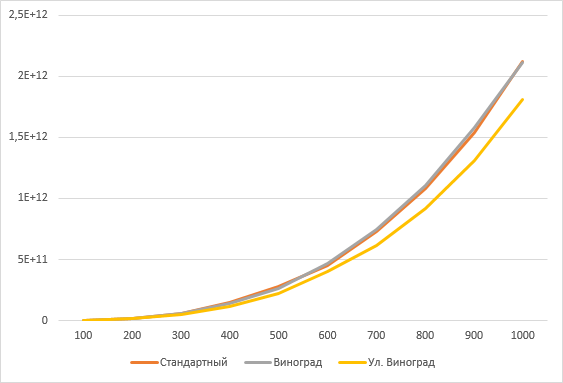
\includegraphics[scale=0.65]{time2.png}
	\captionof{figure}{Зависимость времени выполнения(тики) от размеров таблицы для четной размерности}
	\label{fig:time2}
\end{center}

\begin{center}
	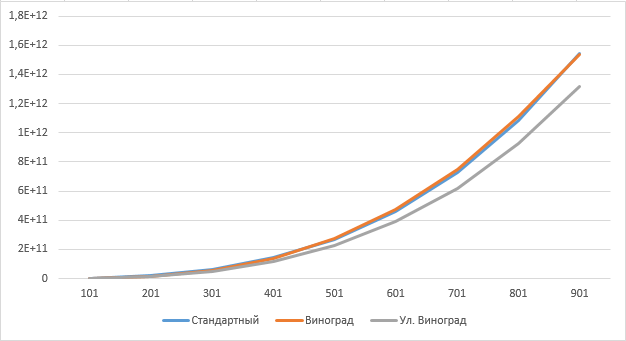
\includegraphics[scale=0.65]{time1.png}
	\captionof{figure}{Зависимость времени выполнения(тики) от размеров таблицы для нечетной размерности}
	\label{fig:time1}
\end{center}

\subsection{Вывод}
\label{sec:exp:conclusion}

Из данных графиков можно сделать вывод, что алгоритм Винограда и классический алгоритм работают приерно одинаково. Также было показано, что произведенные оптимизации алгоритма Винограда улучшили показатели времени работы. 

\newpage
\begin{center}
	\textbf{Заключение}
	\label{sec:outro}
\end{center}

В ходе выполнения лабораторной работы было реализовано два алгоритма перемножения матриц, а также была предложена оптимизация алгоритма Винограда.
Была произведена оценка трудоемкости, показавшая, что алгоритм Винограда более трудоемкий алгоритм, нежели классический алгритм.
Над реализованными методами были проведены ряды тестов, продемонстрировавших правильность их работы. 
Результаты, полученные в экспериментальной части отчета показали, что оптимизация улучшила показатели алгоритма Винограда по времени.  

\newpage
\begin{thebibliography}{9}
	\bibitem{Coppersmith_Winograd} Coppersmith and Shmuel Winograd. «Journal of Symbolic Computation» - М.:  Доклады Академий Наук СССР, 1965.
	\bibitem{Coppersmith_Winograd_2} «Алгоритм Копперсмита — Винограда» [Электронный ресурс]. Journal of Symbolic Computation. – Режим доступа:
	http://ru.math.wikia.com/wiki/Алгоритм Копперсмита — Винограда, свободный.	
	\bibitem{Matrix_Mult} Корн Г., Корн Т. Алгебра матриц и матричное исчисление // Справочник по математике. — 4-е издание. — М: Наука, 1978.  
\end{thebibliography}

\end{document}